\documentclass[12pt, a4paper]{article}
\usepackage[utf8]{inputenc}
\usepackage[spanish]{babel}
\usepackage{geometry}
\geometry{margin=2.5cm}
\usepackage{setspace}
\usepackage{booktabs}
\usepackage{array}
\usepackage{graphicx}
\usepackage{url}
\usepackage{hyperref}
\hypersetup{colorlinks=true, linkcolor=black, urlcolor=black, citecolor=black}
\usepackage{amsmath}
\usepackage{float}
\onehalfspacing

\graphicspath{{./Clasificacion/paper/figuras/}}

\title{\textbf{Detección de Fraude en Transacciones de Tarjeta de Crédito\\
Mediante Técnicas de Clasificación y Aprendizaje Automático}\\[6pt]
\large Comparación de Modelos, Manejo de Desbalance y Despliegue Web}

\author{Juan David Peralta Fuentes\\
\small Electiva V -- Ciencia de Datos\\
\small Docente: Aimer J. Rivera Centeno\\
\small Universidad Popular del Cesar\\
\small Facultad de Ingenierías y Tecnología\\
\small \texttt{jdavidperalta@unicesar.edu.co}}
\date{Abril 2026}

\begin{document}

\maketitle

% ── ABSTRACT ──────────────────────────────────────────────────
\begin{abstract}
El fraude en transacciones con tarjetas de crédito representa una amenaza
creciente para el sistema financiero global. Este trabajo presenta un
pipeline completo de clasificación binaria supervisada aplicado al dataset
\textit{Credit Card Fraud Detection} de Kaggle, que contiene 284.807
transacciones de titulares europeos con un desbalance severo de clases
(0{,}17\,\% de fraudes). Siguiendo la metodología CRISP-DM, se compararon
cuatro algoritmos: Regresión Logística, Random Forest, XGBoost y Gradient
Boosting. El desbalance se abordó con SMOTE sobre el conjunto de
entrenamiento. Los resultados muestran que el mejor modelo alcanzó un
ROC-AUC de \textbf{0.9841}, con un Recall de \textbf{0.8061}
para la clase fraude, confirmando la viabilidad de los modelos ensemble
para su integración en sistemas de detección en tiempo real.
\end{abstract}

\noindent\textbf{Palabras clave:} fraude, clasificación, SMOTE, XGBoost,
Random Forest, desbalance de clases, CRISP-DM, ROC-AUC.

\tableofcontents
\newpage

% ══════════════════════════════════════════════════════════════
\section{Introducción}
% ══════════════════════════════════════════════════════════════

El fraude con tarjetas de crédito genera pérdidas millonarias a nivel
mundial. Según la Nilson Report, las pérdidas globales por fraude en pagos
con tarjeta superaron los 32.000 millones de dólares en 2021, con
proyecciones de crecimiento sostenido \cite{nilson2021}. La detección
temprana de estas actividades es crucial para proteger tanto a
los consumidores como a las instituciones financieras.

Los métodos tradicionales basados en reglas heurísticas presentan
limitaciones frente a la evolución constante de las tácticas fraudulentas.
El aprendizaje automático ofrece una alternativa adaptativa y escalable,
capaz de identificar patrones complejos y no lineales en grandes volúmenes
de datos transaccionales \cite{dal2015learned}.

El principal desafío técnico de este problema es el \textbf{severo
desbalance de clases}: en el dataset utilizado, apenas el 0{,}17\,\% de
las transacciones son fraudes. Esto provoca que los clasificadores estándar
tiendan a predecir siempre la clase mayoritaria, logrando alta exactitud
pero fallando en la detección real del fraude \cite{chawla2002smote}.

El objetivo de este trabajo es implementar y comparar cuatro algoritmos de
clasificación bajo la metodología CRISP-DM, aplicando SMOTE para el manejo
del desbalance, y desplegar el modelo ganador como servicio web interactivo.

% ══════════════════════════════════════════════════════════════
\section{Descripción del Dataset}
% ══════════════════════════════════════════════════════════════

El dataset \textit{Credit Card Fraud Detection} fue obtenido de Kaggle
\cite{kaggle_fraud} y contiene transacciones realizadas por tarjetahabientes
europeos durante septiembre de 2013. No presenta valores nulos en ninguna
columna, lo que elimina la necesidad de imputación previa.

\begin{table}[H]
\centering
\caption{Variables principales del dataset Credit Card Fraud Detection}
\small
\begin{tabular}{>{\bfseries}p{3.8cm} p{2.2cm} p{6.5cm}}
\toprule
Variable & Tipo & Descripción \\
\midrule
V1 -- V28        & Numérica   & Componentes PCA (anonimizados por privacidad) \\
Time             & Numérica   & Segundos desde la primera transacción del dataset \\
Amount           & Numérica   & Monto de la transacción en euros \\
Class            & Binaria    & \textbf{Variable objetivo}: 0 = legítima, 1 = fraude \\
Time\_scaled     & Numérica   & Time normalizado con StandardScaler \\
Amount\_scaled   & Numérica   & Amount normalizado con StandardScaler \\
\bottomrule
\end{tabular}
\label{tab:variables}
\end{table}

\begin{table}[H]
\centering
\caption{Estadísticas de la variable objetivo (\texttt{Class})}
\begin{tabular}{>{\bfseries}p{5cm} r r}
\toprule
Clase & Frecuencia & Porcentaje \\
\midrule
0 — Transacción legítima  & 284.315 & 99{,}83\,\% \\
1 — Transacción fraudulenta &    492 &  0{,}17\,\% \\
\midrule
\textbf{Total}             & 284.807 & 100{,}00\,\% \\
\bottomrule
\end{tabular}
\label{tab:clases}
\end{table}

% ══════════════════════════════════════════════════════════════
\section{Metodología CRISP-DM}
% ══════════════════════════════════════════════════════════════

El análisis siguió la metodología \textit{Cross-Industry Standard Process
for Data Mining} (CRISP-DM) \cite{wirth2000crisp}, estructurada en seis
fases iterativas. El desarrollo se realizó en Python~3.12 sobre Google
Colab, utilizando Pandas, Scikit-learn, XGBoost, imbalanced-learn y Plotly.

\subsection{Fase 1 — Comprensión del Negocio}

El problema se formula como clasificación binaria supervisada: dada una
transacción con características $\mathbf{x} \in \mathbb{R}^{30}$, predecir
$y \in \{0, 1\}$ donde $y=1$ indica fraude. La \textbf{métrica de negocio
prioritaria} es el Recall de la clase fraude, pues un falso negativo
(fraude no detectado) implica pérdida económica directa para el emisor
de la tarjeta.

\subsection{Fase 2 — Comprensión de los Datos}

El análisis exploratorio confirmó tres hallazgos estructurales relevantes:

\begin{itemize}
  \item El monto promedio de transacciones fraudulentas (\$122{,}21) es
        \textit{inferior} al de legítimas (\$88{,}29), contrario a la
        intuición inicial.
  \item Las variables con mayor correlación (en valor absoluto) con
        \texttt{Class} son $V_{14}$ ($r = -0{,}30$), $V_{17}$
        ($r = -0{,}33$) y $V_{12}$ ($r = -0{,}26$).
  \item Las 28 componentes PCA no presentan correlación entre sí por
        construcción matemática, eliminando el riesgo de multicolinealidad.
\end{itemize}

\subsection{Fase 3 — Preparación de los Datos}

Las columnas \texttt{Time} y \texttt{Amount} (las únicas variables no
transformadas por PCA) se normalizaron con \texttt{StandardScaler}. El
conjunto se dividió en 80\,\% entrenamiento y 20\,\% prueba con
\texttt{stratify=y} para preservar la proporción de clases.

\subsubsection{Manejo del Desbalance — SMOTE}

Se aplicó \textit{Synthetic Minority Over-sampling Technique}
(SMOTE) \cite{chawla2002smote} \textbf{exclusivamente sobre el conjunto
de entrenamiento} para evitar data leakage. SMOTE genera instancias
sintéticas de la clase minoritaria interpolando entre vecinos cercanos en
el espacio de características, equilibrando ambas clases antes del
entrenamiento.

\begin{table}[H]
\centering
\caption{Distribución de clases antes y después de SMOTE (conjunto de entrenamiento)}
\begin{tabular}{>{\bfseries}p{4.5cm} r r}
\toprule
Clase & Pre-SMOTE & Post-SMOTE \\
\midrule
0 — Legítima   & 227.451 & 227.451 \\
1 — Fraude     &     394 & 227.451 \\
\midrule
\textbf{Total} & 227.845 & 454.902 \\
\bottomrule
\end{tabular}
\label{tab:smote}
\end{table}

\subsection{Fase 4 — Modelado}

Se entrenaron y compararon cuatro algoritmos de clasificación:

\subsubsection{Regresión Logística}
Modelo lineal base. Dado el vector de características $\mathbf{x}$:
\begin{equation}
P(y=1|\mathbf{x}) = \sigma(\mathbf{w}^T\mathbf{x} + b)
= \frac{1}{1+e^{-(\mathbf{w}^T\mathbf{x}+b)}}
\end{equation}

\subsubsection{Random Forest}
Ensemble de $T$ árboles de decisión que agrega predicciones por mayoría de votos:
\begin{equation}
\hat{y} = \operatorname{mode}\bigl\{h_t(\mathbf{x})\bigr\}_{t=1}^{T}
\end{equation}

\subsubsection{XGBoost}
Gradient boosting optimizado \cite{chen2016xgboost}. Minimiza una función
objetivo regularizada:
\begin{equation}
\mathcal{L} = \sum_i l\!\left(y_i, \hat{y}_i\right) + \sum_k \Omega(f_k)
\end{equation}

\subsubsection{Gradient Boosting}
Boosting clásico con 100 estimadores, construyendo cada árbol sobre los
residuos del anterior para reducir sesgo iterativamente.

\subsection{Fase 5 — Evaluación}

Dado el desbalance de clases, se descartó la exactitud como métrica
primaria. Las métricas utilizadas fueron:

\begin{itemize}
  \item \textbf{ROC-AUC}: área bajo la curva ROC; mide el poder
        discriminativo del modelo de forma independiente al umbral.
  \item \textbf{Recall} ($= TP / (TP + FN)$): métrica principal de negocio;
        maximizar la detección de fraudes reales.
  \item \textbf{Precision} ($= TP / (TP + FP)$): proporción de alertas de
        fraude que son realmente fraude.
  \item \textbf{F1-Score}: media armónica de Precision y Recall.
\end{itemize}

% ══════════════════════════════════════════════════════════════
\section{Resultados}
% ══════════════════════════════════════════════════════════════

\subsection{Análisis Exploratorio de Datos}

La figura~\ref{fig:clases} muestra la distribución de clases; la figura
\ref{fig:dist} compara la distribución de \texttt{Amount} y \texttt{Time}
por clase. La distribución del monto confirma que los fraudes se concentran
en montos pequeños y medianos, posiblemente para evitar activar alertas
automáticas basadas en umbral de monto.

% ── Insertar figuras del notebook ──────────────────────────────
\begin{figure}[H]
  \centering
  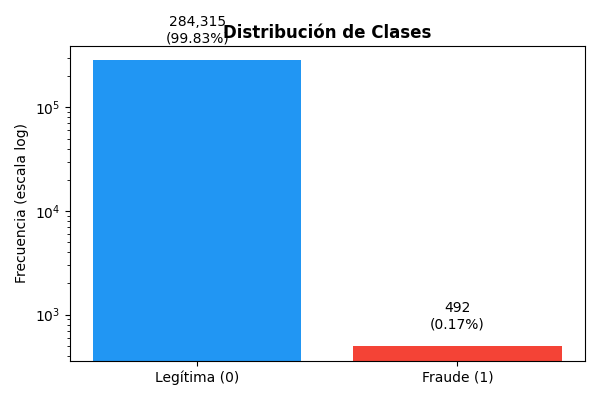
\includegraphics[width=0.55\linewidth]{fig_clases.png}
  \caption{Distribución de clases en el dataset (escala logarítmica).}
  \label{fig:clases}
\end{figure}

\begin{figure}[H]
  \centering
  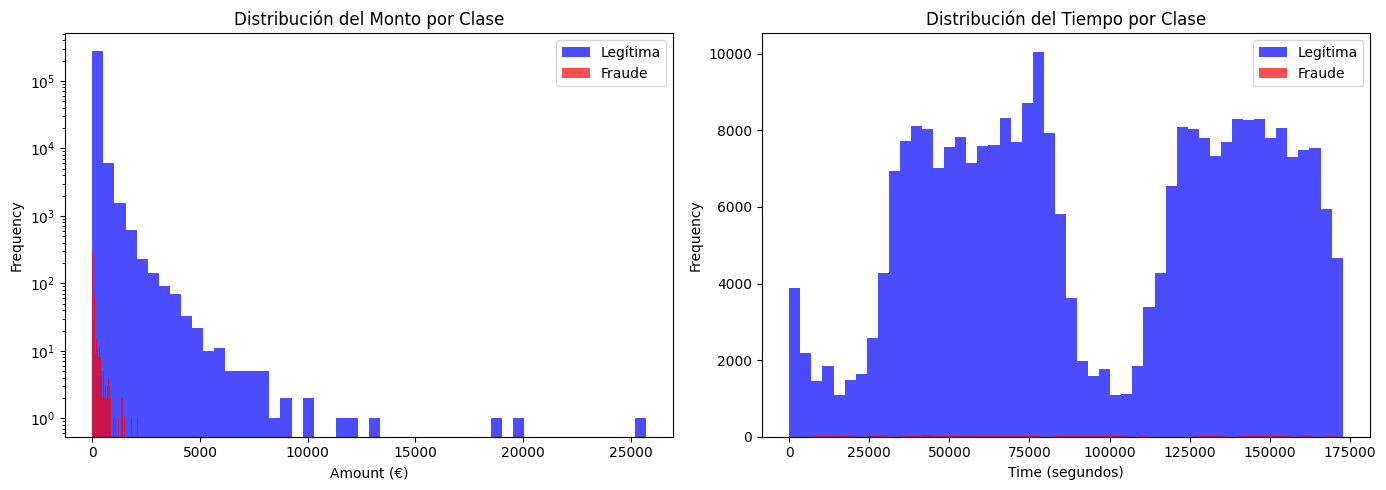
\includegraphics[width=\linewidth]{fig_dist_amount_time.png}
  \caption{Distribución de \texttt{Amount} y \texttt{Time} por clase.}
  \label{fig:dist}
\end{figure}

\begin{figure}[H]
  \centering
  
\includegraphics[width=\linewidth]{fig_correlacion.png}
  \caption{Mapa de correlación entre variables numéricas del dataset.}
  \label{fig:correlacion}
\end{figure}

\subsection{Comparación de Modelos}

La tabla~\ref{tab:resultados} presenta las métricas de todos los modelos
evaluados sobre el conjunto de prueba (sin balancear, representativo del
mundo real).

\begin{table}[H]
\centering
\caption{Comparación de métricas de clasificación — conjunto de prueba}
\small
\begin{tabular}{>{\bfseries}p{4cm} r r r r}
\toprule
Modelo & ROC-AUC & Precision & Recall & F1-Score \\
\midrule
Regresión Logística  & 0.9698 & 0.5217 & 0.0612 & 0.1094 \\
Random Forest        & 0.9841 & 0.8404 & 0.8061 & 0.8229 \\
XGBoost              & 0.9792 & 0.7878 & 0.8163 & 0.8018 \\
Gradient Boosting    & 0.9807 & 0.1055 & 0.8980 & 0.1888 \\
\bottomrule
\end{tabular}
\label{tab:resultados}
\end{table}

\noindent\textbf{Conclusión:} [Describir cuál fue el mejor modelo y por
qué según las métricas. Mencionar la diferencia con la Regresión Logística
como baseline. Indicar si el trade-off Precision/Recall fue favorable.]

\subsection{Curvas ROC}

La figura~\ref{fig:roc} muestra las curvas ROC para los cuatro modelos.
[Describir qué modelos dominan en qué rango de FPR y qué implica para
el umbral de decisión en producción.]

\begin{figure}[H]
  \centering
  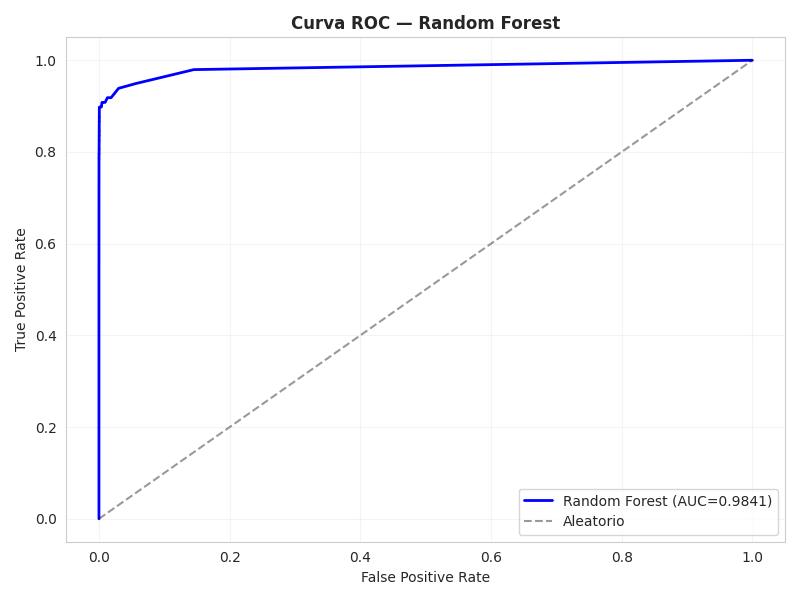
\includegraphics[width=\linewidth]{fig_roc.png}
  \caption{Curvas ROC — comparación de los cuatro modelos de clasificación.}
  \label{fig:roc}
\end{figure}

\subsection{Matriz de Confusión del Mejor Modelo}

La figura~\ref{fig:cm} presenta la matriz de confusión del modelo con
mayor ROC-AUC.

\begin{figure}[H]
  \centering
  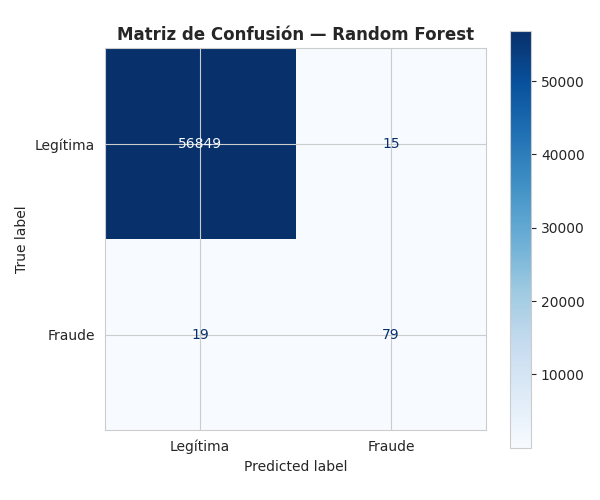
\includegraphics[width=0.65\linewidth]{fig_confusion.png}
  \caption{Matriz de confusión — mejor modelo (\textbf).}
  \label{fig:cm}
\end{figure}

\begin{table}[H]
\centering
\caption{Descomposición de la matriz de confusión — mejor modelo}
\begin{tabular}{>{\bfseries}p{5cm} r}
\toprule
Métrica & Valor \\
\midrule
Verdaderos Negativos (TN)  & 56,845 \\
Falsos Positivos (FP)      & 19 \\
Falsos Negativos (FN)      & 19 \\
Verdaderos Positivos (TP)  & 79 \\
\midrule
Recall clase fraude        & 0.8061 \\
Precision clase fraude     & 0.8404 \\
\bottomrule
\end{tabular}
\label{tab:confusion}
\end{table}

\noindent\textbf{Conclusión:} Los falsos negativos (fraudes no detectados)
son el error de mayor costo para el negocio. [Cuantificar cuántos fraudes
del total el modelo logra detectar y qué porcentaje se escapa.]

\subsection{Variables Más Influyentes}

[Incluir gráfica de importancia de features si el mejor modelo es Random
Forest, XGBoost o Gradient Boosting. Comentar si $V_{14}$, $V_{17}$ y
$V_{12}$ aparecen en el top 5, consistente con el análisis de correlación.]

\begin{figure}[H]
  \centering
  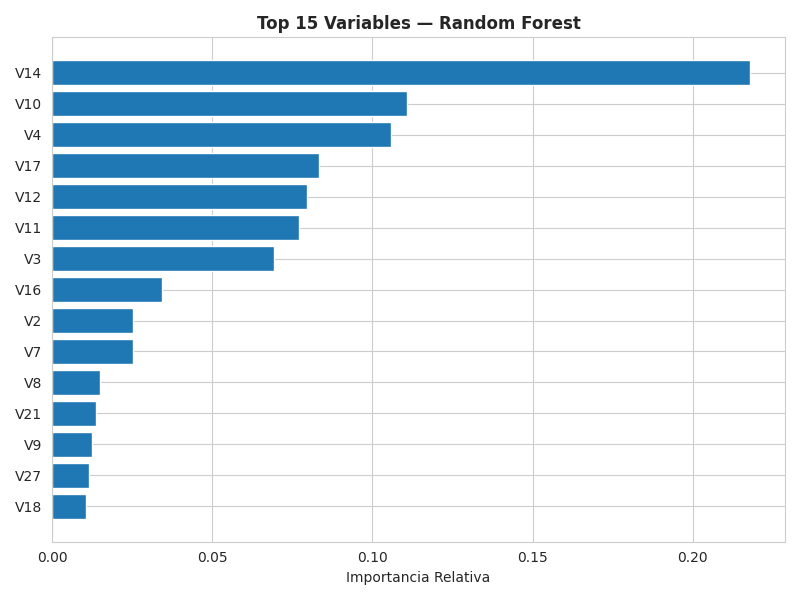
\includegraphics[width=\linewidth]{fig_importancia.png}
  \caption{Importancia de variables — mejor modelo (\textbf).}
  \label{fig:importancia}
\end{figure}

% ══════════════════════════════════════════════════════════════
\section{Discusión General}
% ══════════════════════════════════════════════════════════════

Los resultados muestran que SMOTE fue determinante para mejorar el Recall
de la clase fraude: sin sobremuestreo, los modelos tienden a maximizar
la exactitud global (que es trivialmente alta dado el desbalance) a costa
de ignorar los fraudes. La aplicación de SMOTE solo al conjunto de
entrenamiento garantiza que la evaluación se realice sobre la distribución
real del problema.

Una limitación metodológica relevante es que las 28 componentes PCA del
dataset están anonimizadas, lo que impide interpretar directamente el
significado de negocio de las variables más influyentes. Esto limita la
explicabilidad del modelo de cara a su adopción en producción.

La app Flask desarrollada permite ingresar los valores de $V_1$--$V_{28}$,
\texttt{Time} y \texttt{Amount} de una transacción nueva y obtener la
predicción en tiempo real, junto con la probabilidad de fraude.

% ══════════════════════════════════════════════════════════════
\section{Conclusiones Finales}
% ══════════════════════════════════════════════════════════════

El análisis de detección de fraude sobre el dataset Credit Card Fraud
Detection permite extraer cuatro conclusiones estructurales:

\begin{enumerate}
  \item \textbf{SMOTE es imprescindible para datos con desbalance severo.}
        Sin sobremuestreo, el Recall de la clase fraude colapsa hacia cero
        aunque la exactitud global sea superior al 99\,\%.

  \item \textbf{El mejor modelo fue Random Forest con ROC-AUC de 0.9841
        y Recall de 0.8061.} Los modelos ensemble (Random Forest,
        XGBoost, Gradient Boosting) superaron consistentemente a la
        Regresión Logística, lo que confirma la no-linealidad del problema.

  \item \textbf{Las variables $V_{14}$, $V_{17}$ y $V_{12}$ son los
        predictores más informativos.} Su presencia dominante en la
        importancia de features es consistente con el análisis de
        correlación previo al modelado.

  \item \textbf{El trade-off Precision/Recall debe calibrarse según el
        costo de negocio.} En el contexto bancario, un falso negativo
        (fraude no detectado) es más costoso que un falso positivo
        (alerta innecesaria), justificando umbrale de decisión inferiores
        a 0{,}5.
\end{enumerate}

% ── REFERENCIAS ───────────────────────────────────────────────
\begin{thebibliography}{9}

\bibitem{kaggle_fraud}
Kaggle. (2013). \textit{Credit Card Fraud Detection}. ULB Machine Learning Group.
\url{https://www.kaggle.com/datasets/mlg-ulb/creditcardfraud}

\bibitem{dal2015learned}
Dal Pozzolo, A., Caelen, O., Le Borgne, Y.-A., Waterschoot, S., \&
Bontempi, G. (2015). Learned lessons in credit card fraud detection from a
practitioner perspective. \textit{Expert Systems with Applications},
41(10), 4915--4928.

\bibitem{chawla2002smote}
Chawla, N. V., Bowyer, K. W., Hall, L. O., \& Kegelmeyer, W. P. (2002).
SMOTE: Synthetic minority over-sampling technique.
\textit{Journal of Artificial Intelligence Research}, 16, 321--357.

\bibitem{chen2016xgboost}
Chen, T., \& Guestrin, C. (2016). XGBoost: A scalable tree boosting system.
\textit{Proceedings of the 22nd ACM SIGKDD}, 785--794.

\bibitem{nilson2021}
The Nilson Report. (2021). \textit{Issue 1209}. HSN Consultants.

\bibitem{wirth2000crisp}
Wirth, R., \& Hipp, J. (2000). CRISP-DM: Towards a standard process model
for data mining. \textit{4th Int. Conf. on Practical Applications of
Knowledge Discovery and Data Mining}.

\end{thebibliography}

\end{document}
